\documentclass[10pt,a4paper]{article}
\usepackage[utf8]{inputenc}
\usepackage[italian]{babel}
\usepackage{amsmath}
\usepackage{amsfonts}
\usepackage{amssymb}
\usepackage{graphicx}
\usepackage{gensymb}
\usepackage[left=2cm,right=2cm,top=2cm,bottom=2cm]{geometry}
\newcommand{\rem}[1]{[\emph{#1}]}

\author{Gruppo BN \\ Federico Belliardo, Marco Costa, Lisa Bedini}
\title{Esperienza 10: caratteristiche fisiche porte logiche}
\begin{document}

\maketitle
\section{Scopo dell'esperienza}
Lo scopo dell'esperienza � misurare le caratteristiche statiche e dinamiche delle porte NOT dell'integrato SN74LS04.

\section{Materiale occorrente}
\begin{itemize}
\item IC SN74LS04
\item trimmer da 2 k$\Omega$ e 100 k$\Omega$;
\item Arduino Nano
\item IC SN74LS244
\item trimmer da 10 k$\Omega$
\end{itemize}
\\

\section{Caratteristiche statiche}
Abbiamo montato il circuito come in figura \ref{fig:circuito}.
\begin{figure}
\centering
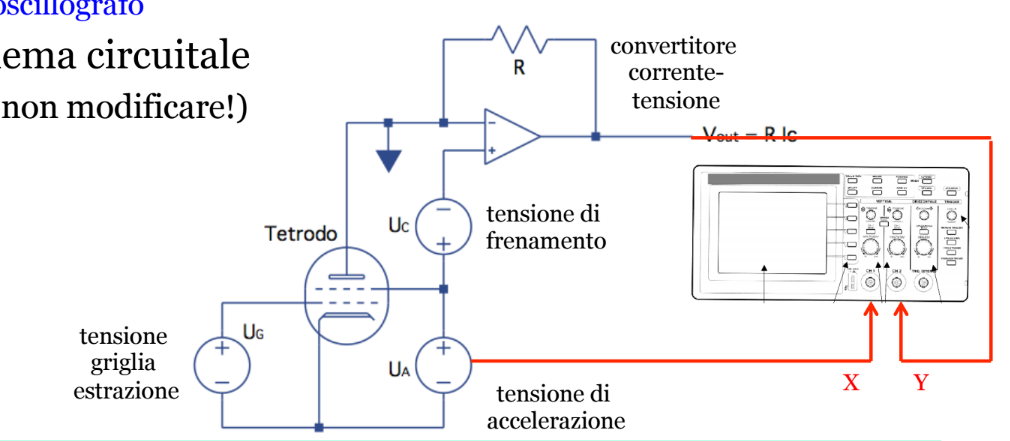
\includegraphics[scale=0.7]{circuito.png}
\caption{Circuito utilizzato\label{fig:circuito}}
\end{figure}
I valori delle componenti sono state misurate tramite multimetro digitale. Come incertezze abbiamo preso quelle riportate sul manuale dello strumento.
Abbiamo misurato la tensione di alimentazione $V_{CC}=4.85\pm 0.03 V$ tramite multimetro digitale (incertezza riportata nel manuale).
%R_trimmer totale = 1950.
%R_1=99.6 ohm
\subsection{Misura delle tensioni di operazione}
Per ottenere diversi valori di $V_{in}$ abbiamo variato opportunamente il trimmer (che ha la funzione di partitore di tensione). Una volta fissata la sua posizione, abbiamo misurato tramite multimetro digitale\footnote{E' lo strumento di misure di tensione in continua con maggiore resistenza interna credo} $V_{in}$ e $V_{out}$.
In tabella \ref{tab:vinvout}e in figura \ref{fig:vinvout}abbiamo riportato le misure ottenute.
\begin{figure}
\centering
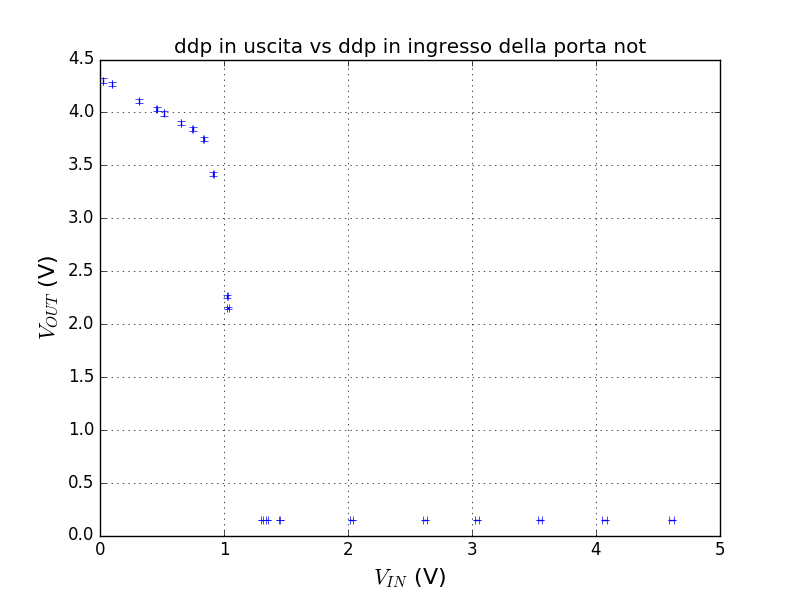
\includegraphics[scale=0.9]{vinvout}
\caption{$V_{out}$ in funzione di $V_{in}$\label{fig:vinvout}}
\end{figure}
\begin{table}
\centering
\begin{tabular}{|c|c|}
\hline

\hline
\end{tabular}
\caption{Misure dei potenziali $V_{in}$, $V_{out}$\label{tab:vinvout}}
\end{table}
Con i dati abbiamo dato una stima dei valori dei potenziali di input/output a livello alto e basso.
La principale incertezza alla determinazione di $V_{IH}$ � dovuta al fatto che in prossimit� di tale valore V_{OUT} varia bruscamente
%manca spiegazione teorica dei valori dei VIO,LH, anche se non penso la chieda...
%devo dire anche quali ho preso...
\subsection{Misura delle correnti in ingresso}
Abbiamo inserito in serie all'ingresso del circuito di figura \ref{fig:circuito} e abbiamo misurato $I_{in}$ al variare di $V_{in}$\footnote{La procedura per variare $V_{in}$ � la stessa del punto precedente}.
%Qua ci va una breve discussio teorica sul verso della corrente e l'andamento)
I dati sono riportati in tabella e in figura.
Dai dati abbiamo stimato i valori di $I_{IH}$ e $I_{IL}$.%Confronto coi valori del datasheet
\subsection{Misura delle correnti in uscita}
Per misurare la massima e minima corrente in uscita dalla porta, abbiamo montato il circuito come in figura \ref{fig:circuito2}\footnote{Il circuito collegato all'ingresso della porta � lo stesso di prima}.
Per la misura di $I_{OL}$ si collega l'uscita a $V_CC$  e si varia il potenziometro $R_1$ in figura \ref{fig:circuito2} in modo che l'uscita sia in stato basso.
Per misurare la corrente abbiamo misurato la caduta di potenziale $V_{ab}$ ai capi della resistenza $R_2$ tramite multimetro digitale. Per verificare che l'uscita fosse effettivamente nello stato basso, si � controllato $V_{out}$ tramite oscilloscopio. Abbiamo deciso di prendere la misura di corrente in corrispondenza del valore di $V_{OL}$ in precedenza. Tuttavia, in questo modo si ottiene $I_{OL}=$, che risulta pi� basso del valore riportato sul datasheet. Abbiamo quindi deciso di prendere una ulteriore misura, in corrispondenza del punto in cui si osservava una brusca variazione di $V_{out}$ e $V_{ab}$. Ci� avviene per V_{out}= e V_{ab}=.
Cos� si ottiene una stima pi� vicina ai valori riportati nel datasheet. Un motivo per cui fallisce il metodo effettuare la misura a V_{OH} stimato � che nelle misure riportate nel grafico \ref{fig:vinvout} non si � riusciti a ottenere misure di V_{out} che non fossero del valore limite 0.144 V.
Per la misura di $I_{OH}$ si collega l'uscita al ground facendo in modo che essa sia in stato alto.
Abbiamo preso la misura in corrispondenza di V_{OUT}=3.7, ossia il valore stimato di V_{OH}.
Cos� si ottiene I_{OH}=, valore in accordo con quanto riportato nel datasheet. La strategia di mettere V_{out} pari alla stima del valore di soglia ottenuto in questo caso funziona meglio perch� i dati del grafico \ref{fig:vinvout} coprono un intorno sufficientemente grande del punto in cui avviene la variazione brusca.

Con questi valori si � dato una stima del \emph{fanout}.
Le correnti che determinano tale valore sono I_{}
e I{IL}.
\section{Montaggio di Arduino}
%R_1=0.98k
%R_2 = 1.003 k 
%R_3 = 0.976 k
%R_4 = 0.989 k
%R_5 = 9.94 k
%C_2 = 106.5 nF
%C_1 = 106.6 nF
Abbiamo montato il circuito in figura \ref{fig:arduino}. Successivamente abbiamo verificato il suo comportamento da generatore di onde quadre. La frequenza del segnale dipende dalla posizione del trimmer. Abbiamo osservato frequenza da , a,. L'ampiezza dell'onda picco-picco � pari a $v_{pp}=$.
In figura \ref{fig:ondaardu} si possono osservare i segnali (misurati tramite oscilloscopio) ai piedini $Y_1$ e $Y_2$.
\section{Caratteristiche dinamiche}
\subsection{Onda in ingresso}
Si � generato tramite Arduino un segnale ad onda quadra di frequenza di circa 1 kHZ e ampiezza XX.
Si � effettuata la misura tramite oscilloscopio\footnote{Le incertezze sono la sensibilit� del cursore pi� il $3\%$ di calibrazione}.

\subsection{Misura dei tempi di propagazione}
Abbiamo eseguito una misura dei due tempi di propagazione, misurando il tempo fra i segnali in ingresso e in uscita fra i due punti a met� della $v_{pp}$ della rampa in salita e discesa rispettivamente\footnote{La misura di tempo � stata eseguita tramite oscilloscopio. Come incertezza si � preso la sensibilit� dei cursori(o la semidispersione se pi� grande in caso di segnale particolarmente rumoroso)}.
I valori riportati nel datasheet sono
$tPHL=8 \mbox{ns}$ e $tPLH= 12 \mbox{ns}$\footnote{valori tipici con resistenza di carico $R_L = 400\Omega$}
\subsection{Misura del tempo di salita}
Con una procedura analoga a sopra, abbiamo misurato il tempo di salita e discesa del segnale in uscita, ossia il tempo necessario per passare dal 10\% della $v_{pp}$ massima al 90\% (Il contrario per il tempo di discesa).
\section{Conclusioni}


\end{document}
